\section{Framework Design}\label{sec:design}
\subsection{The Problem-Solution Abstraction}
Many different types of hard problem we encounter have various input structures. For instance, 3-SAT problem inputs a logic expression while Clique problem needs a graph structure. Those different types of inputs bring the challenge to the CloudCache framework, because it is possible the CloudCache framework hosts many different types of problems and solutions and the cache query operations need to find the exact solutions for a certain problem. If we do not have a uniform structure for all problems, the complexity in localizing problems and its solutions will be very large.

In CloudCache framework, we propose the general \emph{key-value} objects as the abstractions of problem-solutions where problems are the \emph{key} objects and solutions are the \emph{value} objects. To store the key-value objects in the general storage system (e.g. MySQL, Redis and MongoDB), we serialize the keys and values to strings. In this way, the general storage system can easily index, search and maintain the problems and its solutions regardless what type of problem it is.

For a specific problem, like the 3-SAT problem, the developers can define their data structure at their own convenience. The CloudCache framework's cache \emph{query()} and \emph{push()} APIs will first serialize the developer defined data structure when calling both APIs.

\subsection{Core System Design}
\begin{figure}
\centering
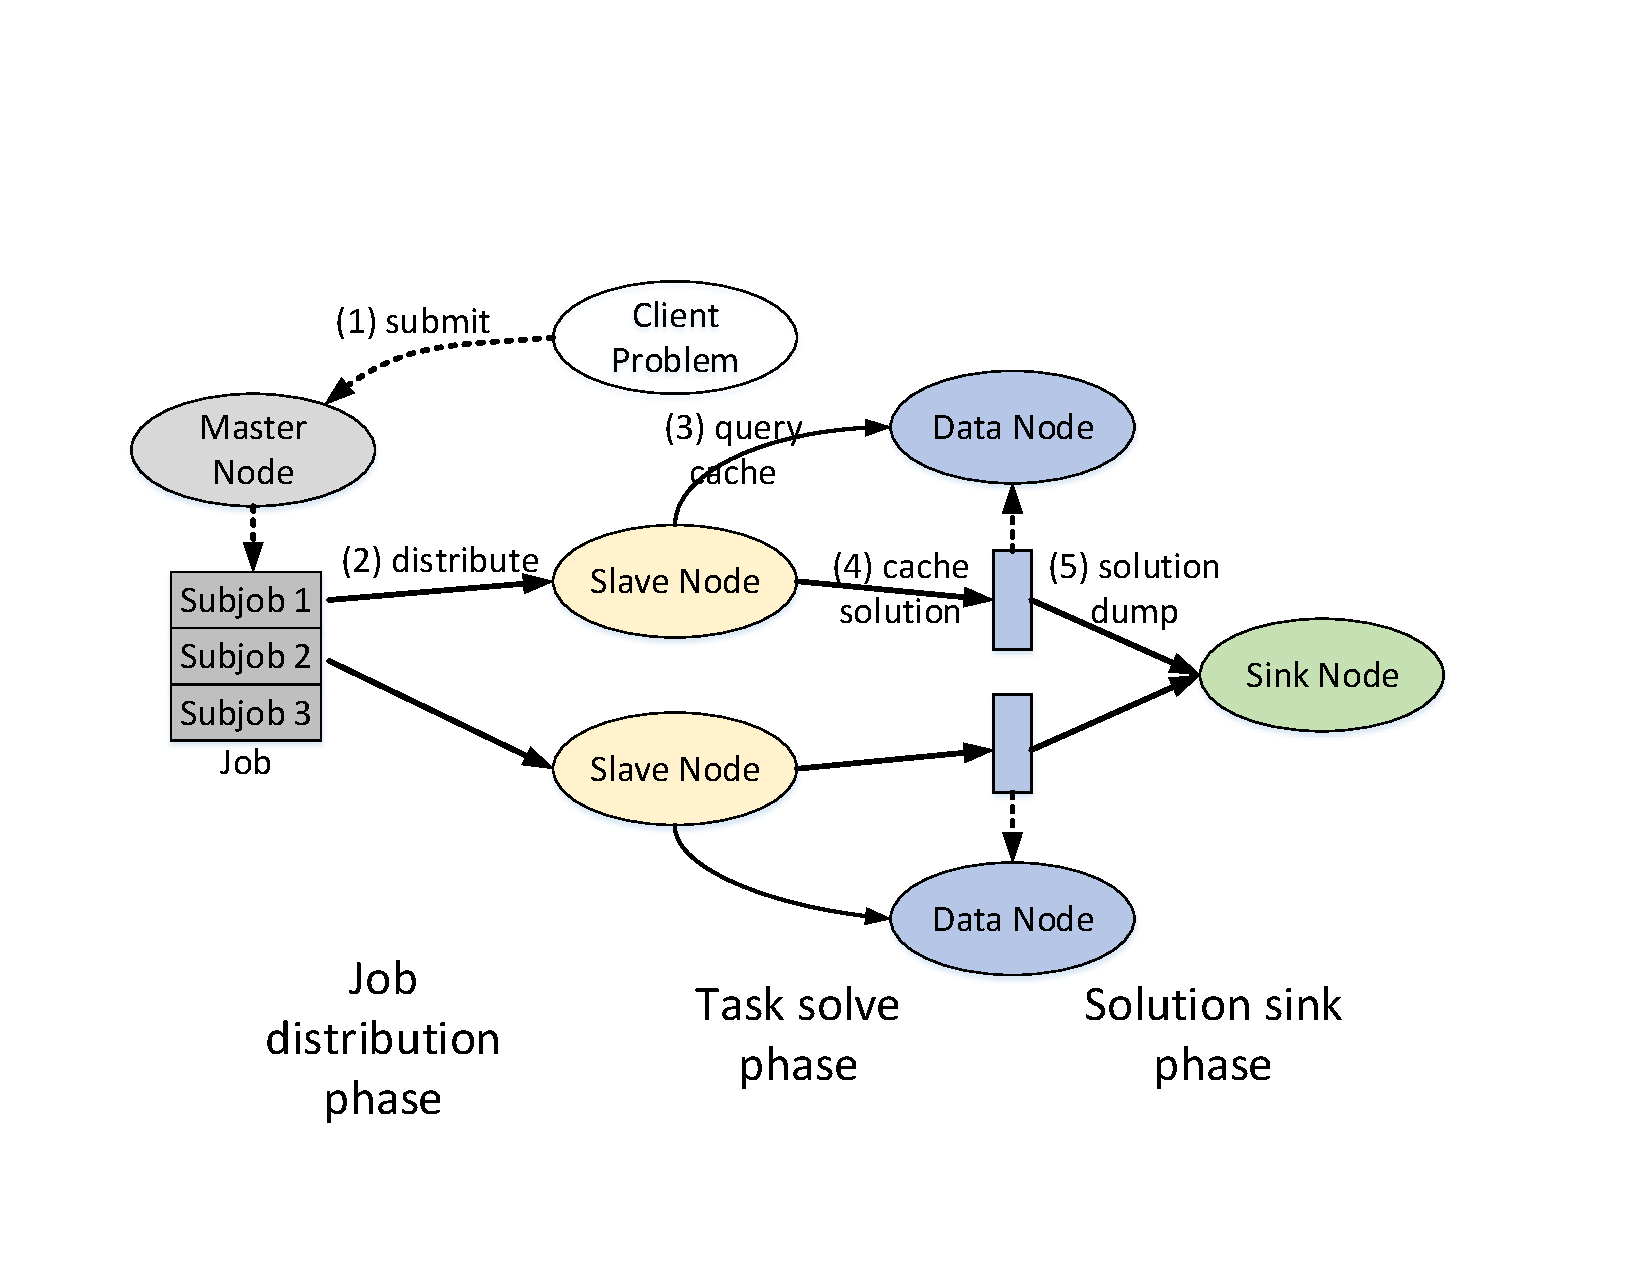
\includegraphics[width=0.45\textwidth]{pics/workflow.pdf}
\caption{The Logic Diagram of CloudCache}
\label{fig:logic}
\end{figure}

The CloudCache framework (Fig.~\ref{fig:logic}) includes four types of nodes and three computation phases in the cloud infrastructure. The nodes are \emph{Master Node}, \emph{Slave Node}, \emph{Data Node} and \emph{Sinker Node}; the three phases are \emph{Job Distribution Phase}, \emph{Task Solve Phase} and \emph{Solution Sink Phase}. In addition, the \emph{Client Problem} exists outside of the cloud infrastructure which needs to be submitted into the CloudCache framework.

The Master Node is the central control component of the whole framework. It accepts the job submission from the client problem and split the the job into several subjobs. Those subjobs will later be distributed to different Slave Nodes. For each of the task in the subjob which the Slave Node is received from the Master Node, the Slave Node will initiate a \emph{kernel-solver} for the task. The kernel-solver is the single execution box defined by the developers for a problem which performs the cache query and solve functions. When the kernel-solver starts execution, it uses the \emph{query()} API to check if the current problem already has a solution in the CloudCache. The query API uses a \emph{hash} function to select the dedicated Data Node where a part of existing solutions are stored. Once the Data Node has been identified, the Data Node will response with a solution if the problem has been solved or a NULL value.

Whether the kernel-solver find the existing solutions or solve it by itself, the solution for the assigned problem will be cached in the Data Node selected by the same hash function. We use a hash function to shard the queries because we consider the load balance of the Data Node, which is much busier than Slave Node or Master Node in the system. In addition to cache the problem's solution, the solution needs to report to the Sinker Node where the client program will come and retrieve the final results for all tasks in the job after the system finishes the job. Note that we only have single Sinker Node while the each kernel-solver will report its results to the Sinker Node, the load at the Sinker Node is significant which defects the whole system's throughput. Therefore, we have a small optimization that buffers the solution in each Slave Node until certain amount, then the Slave Node will report the buffered results together at once.

\subsection{Framework Generalness}
An expected design goal of CloudCache is the generalness, we want to make this framework to be a proper and simple approach to solve many different types of hard problems in the cloud. According to the design, only two things need to be defined by the developer before using the framework. First, the problem and solution's data structure; second, the kernel-solver of the problem, namely when to query the cache and when to solve the problem by itself. After finishing the two parts, the developer can submit a batch of problems as a job to the Master Node, where each problem is regarded as a task. Then the framework will start executing the batch job. In this section, we will show two hard problems' solutions using CloudCache framework.

\subsubsection{3-SAT Problem}
The 3-SAT problem has an input of an boolean expression which contains many boolean variables' combinations in 3-conjunctive-normal-form clauses. For example, Eq.~\ref{eq:3-sat} shows an example 3-SAT problem which has $5$ boolean variables and has three clauses. For this problem, we use the expression vector as the key, but the vector is in a specific format. The boolean variable's index represents the variable itself in the vector, and the the index is set to be negative if the boolean variable has a ``not'' operator. Therefore, the \emph{key} for Eq.~\ref{eq:3-sat} is $[1,2,-3,2,3,4,3,-4,5]$.

\begin{equation}
Y = (x_1 \vee x_2 \vee \overline{x_3}) \wedge (x_2 \vee x_3 \vee x_4) \wedge (x_3 \vee \overline{x_4} \vee x_5)
\label{eq:3-sat}
\end{equation}

On the other hand, the solution of the problem is a vector of assignment, indicating each boolean variable's value as true or false. So for the 3-SAT problem instance in Eq.~\ref{eq:3-sat}, the \emph{value} is $[true, true, false, true, false]$. Once the key-value pair has been designed, we can move on to the \emph{kernel-solver} part.

The kernel-solver has two stages, the first stage is to check if the expression or any subexpression has been solved. We use a linear scan to do it by traversing from the head clause and check the subexpression between the head clause and the end one. For the example in Eq.~\ref{eq:3-sat}, we will check Eq.~\ref{eq:3-sat1},~\ref{eq:3-sat2},~\ref{eq:3-sat3}. If any of the subexpression has been solved, we will retrieve its solution then validate if the assignment can satisfy the whole expression. If so, we do not need a brute-force method to solve it again but just return the assignment in the cache. Otherwise, the brute-force method has to be run and we need to store the solved assignment in the cache. The two simple APIs to query and store key/value in the CloudCache make the operations very easy to do.

Note that we do not enumerate the possible combination of clauses in the expression to query the cache. The major reason is that most of the 3-SAT is not as hard as we may expect, thus the enumeration process may cost more time than a simple brute-force try. Besides, we cannot estimate the cache hit ratio for a clause combination ahead which may make the solution even slower as well.

\begin{equation}
Y = (x_1 \vee x_2 \vee \overline{x_3}) \wedge (x_2 \vee x_3 \vee x_4) \wedge (x_3 \vee \overline{x_4} \vee x_5)
\label{eq:3-sat1}
\end{equation}
\begin{equation}
Y = (x_2 \vee x_3 \vee x_4) \wedge (x_3 \vee \overline{x_4} \vee x_5)
\label{eq:3-sat2}
\end{equation}
\begin{equation}
Y = (x_3 \vee \overline{x_4} \vee x_5)
\label{eq:3-sat3}
\end{equation}


\subsubsection{k-coloring Problem}
The graph's k-coloring problem is to find a color assignment strategy that mark the vertex of the graph so that no adjacent vertex share the same color by using no more than k different colors. The problem is also a classic NP-Complete problem, the exact solution is a brute-force one by enumerating the $k^n$ assignments and validate them.

Similarly, we first need to abstract the problem-solution pairs. For this problem, we use a matrix $\mathbf{R}_{n\times n}$ to represent the graph which is the \emph{key}, and the \emph{value} is the color assignment vector $\mathbf{a} = [a_1, a_2, ..., a_n]$ where $n$ is the number of vertex in the graph.

The kernel-solver also uses a linear scan to all the vertices. For each vertex, we remove the edges connected to the vertex, then we have a new adjacent matrix $\hat{\mathbf{R}}_{(n-1)\times (n-1)}$ which is actually a subgraph of the original one. For this subgraph, we query the CloudCache to retrieve the existing color assignment. If success, we need to validate the assignment by enumerating the color of the removed vertex and combining with the existing solution to see if the complete assignment can fit into the original graph. If so, we can cache the solution; if not, we continue removing another vertex in $\mathbf{R}_{n\times n}$ until we scan all the vertices. If cache is not working at all, the brute-force solver otherwise is triggered. 
